\documentclass[tikz,border=6pt]{standalone}

\usepackage{tikz}
\usetikzlibrary{arrows.meta,positioning,calc}

\begin{document}
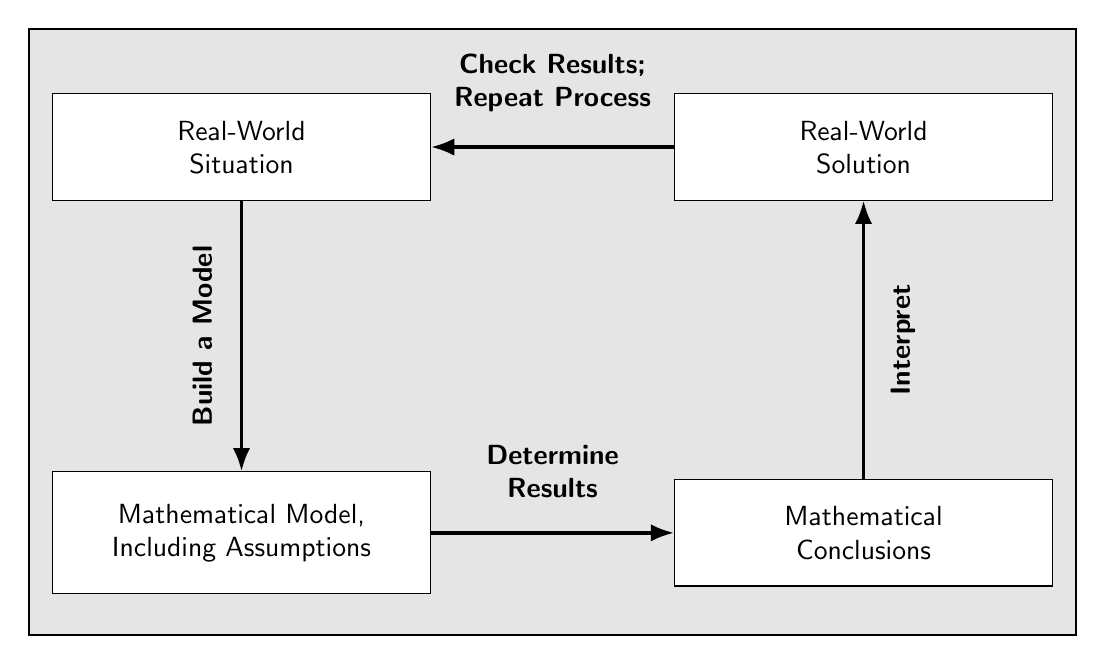
\begin{tikzpicture}[
  font=\sffamily,
  box/.style={draw, fill=white, minimum width=4.8cm, minimum height=1.35cm, align=center},
  arr/.style={-Latex, line width=1.2pt},
  lab/.style={font=\sffamily\bfseries},
  every node/.style={inner sep=6pt}
]

% --- Background + outer frame (like the sample) ---
\fill[black!10] (-1.2,-1.2) rectangle (12.1,6.5);
\draw[black, line width=0.9pt] (-1.2,-1.2) rectangle (12.1,6.5);

% --- Nodes (2×2) ---
\node[box] (rws)   at (1.5,5) {Real-World\\Situation};
\node[box] (rsol)  at (9.4,5) {Real-World\\Solution};

\node[box, minimum height=1.55cm] (mm)  at (1.5,0.1) {Mathematical Model,\\Including Assumptions};
\node[box] (mc) at (9.4,0.1) {Mathematical\\Conclusions};

% --- Arrows + labels ---
% Top: right -> left
\draw[arr] (rsol.west) -- (rws.east)
  node[midway, above=6pt, lab, align=center] {Check Results;\\Repeat Process};

% Left vertical: top -> bottom
\draw[arr] (rws.south) -- (mm.north);
\node[lab, rotate=90] at ($(rws.south)!0.5!(mm.north) + (-0.5,0)$) {Build a Model};

% Bottom: left -> right
\draw[arr] (mm.east) -- (mc.west)
  node[midway, above=6pt, lab, align=center] {Determine\\Results};

% Right vertical: bottom -> top
\draw[arr] (mc.north) -- (rsol.south);
\node[lab, rotate=90] at ($(mc.north)!0.5!(rsol.south) + (0.5,0)$) {Interpret};

\end{tikzpicture}
\end{document}
